% Paper DyBAS-Net, template IEEE hai cột (giống bản thảo PFIN).
% Biên dịch từ thư mục paper/: pdflatex DyBAS-Net && bibtex DyBAS-Net && pdflatex DyBAS-Net && pdflatex DyBAS-Net
% Tên đề tài, nhãn Abstract/Keywords và các đề mục giữ tiếng Anh; nội dung viết tiếng Việt.
% Khung đề mục theo mind map: Abstract (5 câu), I. Introduction (General introduction, Related works,
% Research objective, Structure), II. Methodology (Formulation, Sparse segment, Pattern extraction,
% Dynamic dependency, Proposed model).
\documentclass[conference]{IEEEtran}
\usepackage[utf8]{inputenc}
\usepackage[T5]{fontenc}
\usepackage{cite}
\usepackage{amsmath,amssymb,amsfonts,bm}
\usepackage{graphicx}
\usepackage{booktabs,array,multirow}
\usepackage{pifont}
\usepackage[table]{xcolor}
\usepackage{url}

\renewcommand{\IEEEkeywordsname}{Keywords}

\newcommand{\R}{\mathbb{R}}
\newcommand{\one}{\mathbf{1}}
\newcommand{\LN}{\operatorname{LN}}
\newcommand{\GELU}{\operatorname{GELU}}
\newcommand{\DF}{\operatorname{DF}}
\newcommand{\FFN}{\operatorname{FFN}}
\newcommand{\vecr}{\operatorname{vec}}
\newcommand{\cmark}{\ding{51}}
\newcommand{\xmark}{\ding{55}}

\begin{document}

\title{Dynamic Dependency Learning and Sparse Segment-Based Pattern Extraction for Multivariate Time Series Load
Forecasting}

\author{
\IEEEauthorblockN{1\textsuperscript{st} Nguyen Thi Ngoc Anh}
\IEEEauthorblockA{\\ \\ \\}
\and
\IEEEauthorblockN{2\textsuperscript{nd} Nguyen Hai Long}
\IEEEauthorblockA{\\ \\ \\}
\and
\IEEEauthorblockN{3\textsuperscript{rd} Bui Hoang Tien Dat}
\IEEEauthorblockA{\\ \\ \\}
}

\maketitle

%=====================================================================
\begin{abstract}
Dự báo phụ tải đa biến cần khai thác đồng thời tính lặp lại có chu kỳ của từng chuỗi và sự phụ thuộc giữa các biến vốn
thưa và thay đổi theo thời gian, trong khi xu hướng dùng cửa sổ quá khứ dài khiến chi phí tính toán của các mô hình dự
báo ngày càng lớn.
Bài báo đề xuất DyBAS-Net, mô hình chia mỗi chuỗi thành các đoạn dài bằng một chu kỳ, nén chúng thành một số ít đoạn cơ
sở, rồi học phụ thuộc thưa và động giữa các biến trực tiếp trên các đoạn cơ sở này bằng một nhánh trộn kênh dùng
DropFusion, có đầu ra khởi tạo bằng không để hiệu chỉnh các cơ sở trước khi dự báo theo đoạn.
Mục tiêu là bổ sung khả năng mô hình hóa liên biến cho một bộ dự báo theo đoạn độc lập kênh siêu nhẹ, mà vẫn giữ chi phí
tính toán thấp và không làm mô hình kém đi so với backbone lúc khởi tạo.
Thực nghiệm trên các bộ dữ liệu chuẩn và dữ liệu phụ tải cho thấy nhánh trộn kênh cải thiện độ chính xác của backbone
trên mọi bộ dữ liệu, và DyBAS-Net đạt độ chính xác cạnh tranh với các mô hình hiện đại trong khi chi phí suy luận cùng
bậc với các mô hình tuyến tính và thấp hơn nhiều lần so với các mô hình học sâu.
Ưu điểm của mô hình là vừa nhẹ vừa tận dụng được thông tin liên biến; hạn chế là mức cải thiện so với backbone còn khiêm
tốn khi phụ thuộc giữa các biến yếu, và mức độ thưa của DropFusion cần được chọn riêng cho từng bộ dữ liệu.
\end{abstract}

\begin{IEEEkeywords}
Dynamic dependency, Sparse segment, Multivariate time series, Load forecasting, Pattern extraction
\end{IEEEkeywords}

%=====================================================================
\section{Introduction}

\subsection{General Introduction}

Dự báo phụ tải được xem là năng lực nền tảng cho quy hoạch và vận hành hệ thống điện~\cite{Hong2016Probabilistic}, và các
hệ thống được quan sát thường là đa biến: một máy biến áp ghi nhận phụ tải cùng với nhiệt độ dầu, một công ty điện lực
ghi nhận cùng lúc lượng tiêu thụ của hàng trăm khách hàng. Vì vậy, dự báo chuỗi thời gian đa biến (MTSF) phải dự báo
đồng thời tất cả các biến, và việc nắm bắt phụ thuộc giữa các kênh đồng thời xử lý sự dịch chuyển phân phối ngày càng
khó khăn khi quy mô và lĩnh vực ứng dụng mở rộng~\cite{Kim2025Survey}.

Hình~\ref{fig:intro} minh họa hai tính chất của loại dữ liệu này trên phụ tải điện Hà Nội. Thứ nhất là \emph{sự lặp lại
có chu kỳ}: các đoạn ngày gần như trùng hình dạng (Hình~\ref{fig:intro}a, b), và khi xếp $L=720$ giờ thành $N=30$ đoạn
ngày, mọi ngày có thể dựng lại từ chỉ 6 ``ngày điển hình'' với sai số 3,5\% (Hình~\ref{fig:intro}c). Tính hạng thấp này
cho phép TimeBase dự báo chỉ
với 0,39K tham số~\cite{Huang2025TimeBase}, và dữ liệu điện nói chung có một mẫu hình ngày dùng chung~\cite{Lin2024CycleNet}.
Thứ hai là \emph{phụ thuộc giữa các biến thay đổi theo trạng thái}: tương quan giữa phụ tải sinh hoạt và nhiệt độ dương
mạnh trong phần lớn thời gian nhưng đổi dấu, chủ yếu vào tháng 1 và tháng 3 (Hình~\ref{fig:intro}d). Điều này khớp với
nhận xét rằng cùng một cặp biến có thể liên kết mạnh ở chế độ này nhưng yếu ở chế độ khác~\cite{Zhang2026MSFLOW}, và
tương quan trên từng mẫu có thể khác đáng kể tương quan toàn cục~\cite{Lin2025TQNet}. Vì vậy, mô hình độc lập kênh (CI)
bền vững nhưng bỏ qua tương tác, còn mô hình phụ thuộc kênh (CD) nắm được tương tác nhưng nhạy với nhiễu từ các kênh
không liên quan~\cite{Han2024Capacity,Qiu2025DUET}.

\begin{figure*}[t]
\centering
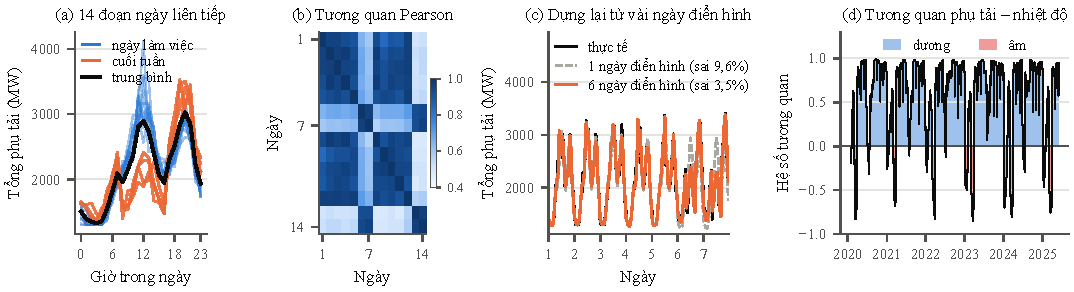
\includegraphics[width=\textwidth]{figures/intro_load.pdf}
\caption{Hai tính chất của dữ liệu phụ tải điện Hà Nội (theo giờ, 01/2020--05/2025). (a) 14 ngày liên tiếp của tổng phụ
tải (từ 06/03/2023) chồng lên nhau. (b) Tương quan Pearson giữa 14 đoạn ngày đó; các ngày cuối tuần (6--7 và 13--14) tạo
khối riêng, cho thấy thêm chu kỳ tuần. (c) Xếp $L=720$ giờ thành ma trận $N\times P=30\times24$ rồi biểu diễn mỗi ngày
bằng tổ hợp tuyến tính của $R$ ``ngày điển hình'' (xấp xỉ hạng $R$); hình vẽ 7 ngày đầu của cửa sổ, sai số tương đối
trung bình trên mọi cửa sổ ghi trong chú giải. Một ngày điển hình bỏ sót cuối tuần, còn $R=6$ gần như trùng số liệu
thật. (d) Tương quan cuộn 30 ngày giữa phụ tải sinh hoạt và hệ số nhiệt độ, dao động từ $-0{,}85$ đến $0{,}99$.}
\label{fig:intro}
\end{figure*}

Đồng thời, xu hướng dùng cửa sổ quá khứ rất dài (ví dụ $L=720$) làm tăng số tham số và khối lượng tính toán của các bộ
dự báo~\cite{Huang2025TimeBase}. Do đó, một bộ dự báo phụ tải thực tiễn cần (i) đủ nhẹ để triển khai trên thiết bị hạn
chế tài nguyên, (ii) khai thác được các mẫu hình chu kỳ, và (iii) học được phụ thuộc giữa các biến mà không khuếch đại các
phụ thuộc giả. Mục tiếp theo cho thấy các phương pháp hiện có chỉ đáp ứng tối đa hai trong ba yêu cầu này.

\subsection{Related Works}

Các công trình liên quan được tổ chức theo năm từ khóa của bài báo. Với mỗi chủ đề, chúng tôi nêu bài toán mà chủ đề giải
quyết, điểm qua các công trình tiêu biểu, so sánh chúng, chỉ ra ưu điểm, nhược điểm và khoảng trống mà DyBAS-Net hướng tới.

\subsubsection{Sparse segment}
Hướng nghiên cứu này thay việc mô hình hóa trục thời gian theo từng điểm bằng các phép toán trên đoạn (patch hoặc chu kỳ).
PatchTST chia mỗi chuỗi đơn biến thành các patch mức chuỗi con, dùng làm token cho Transformer và chia sẻ mô hình giữa các
kênh~\cite{Nie2023PatchTST}. TimesNet biến đổi chuỗi 1D thành các tensor 2D theo các chu kỳ của nó, để biến thiên trong
chu kỳ và giữa các chu kỳ được nắm bắt bằng tích chập 2D~\cite{Wu2023TimesNet}. WITRAN truyền thông tin theo kiểu sóng
nước ở hai mức độ chi tiết để nắm các mẫu lặp dài hạn và ngắn hạn, kèm mạng hồi tiếp tăng tốc cho dự báo
tầm xa~\cite{Jia2023WITRAN}. CFPT mô hình hóa tương tác liên tần số cùng với
dấu thời gian nhận biết chu kỳ~\cite{Kou2025CFPT}, và các mạng tương tác đa chu kỳ mô hình hóa tường minh tương tác giữa
nhiều thành phần chu kỳ~\cite{Xie2025MPIN}; việc mô hình hóa tương tác tường minh như vậy được ghi nhận là cải thiện đáng
kể độ chính xác~\cite{Kou2025CFPT,Xie2025MPIN}. So sánh với nhau, PatchTST dùng patch có độ dài cố định, còn TimesNet
và các mô hình đa chu kỳ tổ chức chuỗi theo chu kỳ của dữ liệu. Ưu điểm của chúng là token mức đoạn bền vững hơn
với nhiễu cục bộ và rút ngắn chuỗi cần xử lý. Nhược điểm là các đoạn được đưa vào các backbone sâu (Transformer, tích chập
hoặc hồi tiếp), nên việc giảm độ dài chuỗi không dẫn đến một mô hình nhỏ. Trường hợp cực đoan của tính thưa mức đoạn, tức dự báo hoàn toàn tuyến
tính giữa các chu kỳ (SparseTSF~\cite{Lin2024SparseTSF}) hoặc trên một số ít đoạn cơ sở
(TimeBase~\cite{Huang2025TimeBase}), cực kỳ nhẹ nhưng xử lý mỗi biến một cách độc lập. Khoảng trống là một biểu diễn mức
đoạn gọn như TimeBase nhưng vẫn trao đổi được thông tin giữa các biến.

\subsubsection{Multivariate time series}
MTSF nhằm mô hình hóa đồng thời nhiều biến phụ thuộc lẫn nhau~\cite{Kim2025Survey}. Các thiết kế tiêu biểu học biểu diễn
tổng quát bằng học tương phản~\cite{Hu2023Contrastive}, tăng cường phân tích mùa vụ--xu hướng bằng nhiều
wavelet~\cite{Zhang2025MWENet}, hợp nhất dữ liệu đa thang đo bằng mạng Kolmogorov--Arnold với hàm mất mát thích
nghi~\cite{Liu2026MSDFKAN}, và kết hợp biểu diễn miền thời gian và miền tần số trong một Transformer~\cite{Chen2024JTFT}.
Các Transformer trước đó cải thiện hiệu quả của attention trên chuỗi dài (Informer~\cite{Zhou2021Informer}) hoặc tích hợp
phân rã với cấu trúc miền tần số (FEDformer~\cite{Zhou2022FEDformer}); JTFT còn dùng một lớp attention hạng thấp để nắm
phụ thuộc giữa các chiều~\cite{Chen2024JTFT}. So sánh với nhau, các mô hình này khác nhau chủ yếu ở cách biểu diễn tín
hiệu thời gian (embedding tương phản, wavelet, hợp nhất đa thang đo, token thời gian--tần số), nhưng cùng dựa trên một
mạng sâu (Transformer, mạng wavelet, KAN). Ưu điểm của chúng là khả năng biểu diễn mạnh đối với động học phức tạp, phi
tuyến. Nhược điểm, theo đánh giá của chúng tôi, là chi phí của backbone sâu lớn hơn nhiều so với một ánh xạ tuyến tính,
và quan hệ liên biến được học lẫn trong backbone thay vì qua một cơ chế thưa, tường minh. Khoảng trống là một mô hình đa
biến có thành phần liên biến thưa và thành phần thời gian rẻ như một ánh xạ tuyến tính.

\subsubsection{Load forecasting}
Dự báo phụ tải dự đoán nhu cầu điện hoặc năng lượng của tòa nhà, khách hàng và lưới điện. Dự báo phụ tải xác suất đã được
hệ thống hóa trong các bài tổng quan dạng hướng dẫn, tóm tắt kỹ thuật, tiêu chuẩn đánh giá và những ngộ nhận
phổ biến~\cite{Hong2016Probabilistic}. Các mô hình đa mùa vụ cổ điển vẫn được dùng rộng rãi: một mô hình ARIMA đa mùa vụ
thích nghi dự báo phụ tải nước nóng sinh hoạt~\cite{Nagpal2025ARIMA}, và SARIMA kết hợp phân tích phổ các thành phần chu
kỳ được dùng để dự báo nhu cầu điện đỉnh theo mùa~\cite{MelchorCruz2025Spectral}. Tuy vậy, các cách tiếp cận cổ điển như
phân rã Fourier, làm trơn mũ và SARIMA chưa phản ánh đặc trưng riêng của từng chu kỳ mùa vụ cũng như tương tác giữa
chúng~\cite{Moon2022MixedPooling}. Về phía học sâu, DeepAR học một mạng hồi tiếp (RNN) tự hồi quy toàn cục trên
nhiều chuỗi liên quan và đưa ra toàn bộ phân phối dự báo~\cite{Salinas2020DeepAR}, còn Temporal Fusion Transformer kết hợp
cơ chế chọn biến với attention có thể diễn giải cho dự báo đa tầm với biến đồng hành tĩnh, đầu vào tương lai đã biết và
tín hiệu lịch sử~\cite{Lim2021TFT}. Các mô hình thống kê minh bạch và rẻ, nhưng dựa trên giả định tuyến tính cứng nhắc và
thường xử lý các thành phần mùa vụ riêng rẽ; các mô hình sâu nắm bắt được tính phi tuyến và chia sẻ thông tin giữa các
chuỗi, nhưng nặng và không mô hình hóa tường minh việc khách hàng hay cảm biến nào ảnh hưởng lẫn nhau. Khoảng trống là
một bộ dự báo phụ tải giữ cấu trúc chu kỳ tường minh như các mô hình cổ điển, đồng thời học được các hiệu ứng phi tuyến
và liên biến với chi phí nhỏ.

\subsubsection{Dynamic dependency}
Chủ đề này quan tâm đến cách học phụ thuộc giữa các biến khi chúng thưa, nhiễu và thay đổi theo thời gian. MS-FLOW xem
tương tác liên biến là một dòng thông tin có dung lượng giới hạn: mô hình gộp các token patch thành trạng thái mức biến,
chỉ giữ Top-$K$ logit tương đồng cho mỗi biến trong một đồ thị thích nghi theo mẫu, và lan truyền thông tin dọc các cạnh
này~\cite{Zhang2026MSFLOW}. xCPD xem mỗi cặp kênh--patch là một nút đồ thị, chiếu các nút lên một cơ sở Fourier đồ thị
dùng chung, nhóm chúng thành các dải tần thấp, trung và cao, rồi định tuyến mỗi patch tới các bộ lọc theo tần số bằng
mixture of experts động; xCPD được dùng như một mô-đun cắm thêm trên backbone CI hoặc CD~\cite{Li2026xCPD}. DUET phân cụm
mềm các kênh trong miền tần số bằng metric Mahalanobis học được và mặt nạ lấy mẫu Bernoulli, rồi hợp nhất kết quả với đặc
trưng thời gian qua masked attention~\cite{Qiu2025DUET}. TQNet dùng các vector học được dịch chuyển theo chu kỳ làm query
và đầu vào gốc làm key và value, để một lớp attention duy nhất kết hợp tương quan toàn cục và tương quan mức
mẫu~\cite{Lin2025TQNet}. Cả bốn công trình đều thống nhất rằng việc trộn dày đặc, không giới hạn sẽ lan truyền nhiễu:
MS-FLOW báo cáo biến thể dày đặc kém hơn định tuyến Top-$K$~\cite{Zhang2026MSFLOW}, và DUET báo cáo attention đầy đủ làm
giảm độ chính xác trên ETTh2~\cite{Qiu2025DUET}. Chúng khác nhau ở chỗ áp đặt tính thưa (cạnh Top-$K$, dải phổ, cụm mềm,
query chu kỳ). Ưu điểm của chúng là mô hình hóa phụ thuộc bền vững, trong đó TQNet và xCPD còn chú trọng hiệu quả tính
toán. Nhược điểm là phụ thuộc được học trên token mức patch hoặc mức điểm, nên đồ thị hoặc attention tăng theo số biến $C$
(ma trận khoảng cách, xác suất và mặt nạ kích thước $C\times C$ giữa mọi cặp kênh trong DUET~\cite{Qiu2025DUET}, đồ thị
có nút là mọi cặp kênh--patch trong
xCPD~\cite{Li2026xCPD}); MS-FLOW cần chọn ngân sách thưa $K$ theo từng bộ dữ liệu, dù không quá nhạy với
$K$~\cite{Zhang2026MSFLOW}, và TQNet lưu ý
rằng việc ép mô hình hóa đa biến mạnh có thể gây hại khi tương quan yếu~\cite{Lin2025TQNet}. Khoảng trống là học phụ thuộc
thưa trên một biểu diễn nhỏ hơn nhiều so với chuỗi patch, được gắn vào sao cho không thể làm backbone kém đi.

\subsubsection{Pattern extraction}
Chủ đề này quan tâm đến cách trích xuất và tái sử dụng các mẫu hình lặp lại cho dự báo. CycleNet học các chu kỳ lặp
$Q\in\R^{W\times C}$ với độ dài chu kỳ $W$ dùng chung cho cả bộ dữ liệu, loại chúng khỏi đầu vào và chỉ dự báo phần
dư; mô-đun này chỉ thêm $W\times C$ tham số và không thêm phép nhân--cộng nào~\cite{Lin2024CycleNet}. TimeEmb tách thành
phần bất biến theo thời gian, được truy xuất từ một ngân hàng embedding học được đánh chỉ số theo dấu thời gian, khỏi thành
phần biến đổi theo thời gian được xử lý bằng bộ lọc tần số~\cite{Xia2025TimeEmb}. GTR duy trì một embedding thời gian toàn
cục cho cả một chu kỳ, truy xuất đoạn khớp với vị trí tuyệt đối của đầu vào và hợp nhất nó với đầu vào qua tích chập 2D;
mô-đun chỉ cần 40,1K tham số~\cite{Cao2026GTR}. LightGTS cắt chuỗi thành các patch có độ dài bằng độ dài chu kỳ, để mỗi
token bao phủ trọn một chu kỳ nội tại trên các bộ dữ liệu có thang thời gian khác nhau, và giải mã song song các giá trị
tương lai~\cite{Wang2025LightGTS}. So sánh với nhau, CycleNet, TimeEmb và GTR lưu các mẫu hình \emph{toàn cục} học trên
cả tập huấn luyện, còn LightGTS trích xuất các mẫu hình \emph{cục bộ} căn theo chu kỳ từ cửa sổ đầu vào. Ưu điểm chung là
cấu trúc chu kỳ được nắm bắt với chi phí thấp: CycleNet không thêm phép nhân--cộng~\cite{Lin2024CycleNet}, TimeEmb là một
khung phân rã gọn nhẹ~\cite{Xia2025TimeEmb}, và LightGTS nhỏ hơn 10--100 lần các mô hình nền tảng
khác~\cite{Wang2025LightGTS}. Nhược điểm chung là các mẫu hình được trích xuất theo từng
kênh: CycleNet thua iTransformer trên Traffic và nêu việc mô hình hóa liên kênh là hướng phát triển
tương lai~\cite{Lin2024CycleNet}, còn GTR cần thêm một mô-đun tổng hợp token toàn cục để cải thiện MSE trên Traffic
8,8--10,4\%~\cite{Cao2026GTR}. Khoảng trống là cho chính các mẫu hình đã trích xuất tương tác với nhau giữa các biến.

\subsubsection{Research gap}
Bảng~\ref{tab:gap} tổng hợp năm chủ đề. Các phương pháp dựa trên đoạn và trích xuất mẫu hình thì nhẹ và khai thác được
tính chu kỳ, nhưng mô hình hóa mỗi biến độc lập hoặc dựa vào backbone nặng. Các phương pháp phụ thuộc động học được quan
hệ liên biến thưa và thích nghi, nhưng trên token mức patch hoặc mức điểm có số lượng tăng theo đầu vào, nên không nhẹ
bằng các mô hình tuyến tính mức đoạn. Thực tiễn dự báo phụ tải bị chia giữa các mô hình thống kê minh bạch nhưng tuyến
tính và các mô hình sâu phi tuyến nhưng nặng. Theo hiểu biết của chúng tôi, chưa có mô hình nào \emph{vừa} giữ được chi phí
của một bộ dự báo mức đoạn siêu nhẹ \emph{vừa} học được phụ thuộc liên biến thưa và động, cũng chưa có phương pháp nào
học các phụ thuộc này trực tiếp trên các mẫu hình chu kỳ đã trích xuất (các đoạn cơ sở) theo cách giữ nguyên backbone CI
tại thời điểm khởi tạo.

\begin{table*}[t]
\caption{So sánh các hướng tiếp cận liên quan theo ba yêu cầu của một bộ dự báo phụ tải đa biến thực tiễn.}
\label{tab:gap}
\centering
\small
\renewcommand{\arraystretch}{1.15}
\resizebox{\textwidth}{!}{%
\begin{tabular}{@{}llccc@{}}
\toprule
Nhóm phương pháp & Công trình tiêu biểu & Biểu diễn chu kỳ / đoạn & Phụ thuộc liên biến & Gọn nhẹ\\
\midrule
Đoạn thưa, tuyến tính & SparseTSF~\cite{Lin2024SparseTSF}, TimeBase~\cite{Huang2025TimeBase}
  & \cmark\ chu kỳ, đoạn cơ sở & \xmark\ (CI) & \cmark\\
Mô hình sâu theo đoạn & PatchTST~\cite{Nie2023PatchTST}, TimesNet~\cite{Wu2023TimesNet}, WITRAN~\cite{Jia2023WITRAN}
  & \cmark\ patch, chu kỳ 2D, mẫu lặp hai mức & \xmark\ / ngầm định & \xmark\\
Mô hình sâu đa biến & Informer~\cite{Zhou2021Informer}, FEDformer~\cite{Zhou2022FEDformer},
  JTFT~\cite{Chen2024JTFT}, iTransformer~\cite{Liu2024iTransformer} & \xmark\ điểm, token tần số
  & \cmark\ dày đặc / hạng thấp (JTFT) & \xmark\\
Mô hình phụ tải thống kê & ARIMA đa mùa vụ~\cite{Nagpal2025ARIMA}, SARIMA kết hợp phân tích phổ~\cite{MelchorCruz2025Spectral}
  & \cmark\ thành phần mùa vụ & \xmark & \cmark\ (tuyến tính)\\
Mô hình phụ tải học sâu & DeepAR~\cite{Salinas2020DeepAR}, TFT~\cite{Lim2021TFT} & \xmark & chỉ qua biến đồng hành & \xmark\\
Trích xuất mẫu hình & CycleNet~\cite{Lin2024CycleNet}, TimeEmb~\cite{Xia2025TimeEmb}, GTR~\cite{Cao2026GTR},
  LightGTS~\cite{Wang2025LightGTS} & \cmark\ chu kỳ toàn cục, token chu kỳ & \xmark\ (CI) & \cmark\\
Phụ thuộc thưa / thích nghi & MS-FLOW~\cite{Zhang2026MSFLOW}, xCPD~\cite{Li2026xCPD}, DUET~\cite{Qiu2025DUET}
  & patch, cặp kênh--patch & \cmark\ thưa, thích nghi & một phần\\
Attention với query chu kỳ & TQNet~\cite{Lin2025TQNet} & \cmark\ query chu kỳ & \cmark\ attention & một phần\\
\midrule
\rowcolor{gray!15}
\textbf{DyBAS-Net (đề xuất)} & -- & \cmark\ đoạn cơ sở & \cmark\ thưa, động, trên cơ sở & \cmark\\
\bottomrule
\end{tabular}}
\end{table*}

\subsection{Research Objective}

Bài báo đề xuất \textbf{DyBAS-Net} (\textbf{Dy}namic cross-variable dependency on \textbf{BAS}is segments) với các mục
tiêu sau:
\begin{itemize}
  \item \emph{Trích xuất mẫu hình dựa trên đoạn thưa.} Phân đoạn mỗi chuỗi theo chu kỳ tự nhiên, chuẩn hóa từng pha và
        nén $N$ đoạn quá khứ thành $R\ll N$ đoạn cơ sở trực giao.
  \item \emph{Học phụ thuộc động trong không gian cơ sở.} Học phụ thuộc giữa các biến bằng CrossVBlock, DropFusion và
        IntraVBlock của DyTimeNet~\cite{Chen2026DyTimeNet}, áp dụng trên $P\cdot R$ hệ số cơ sở của mỗi biến thay vì
        $L$ điểm gốc.
  \item \emph{Hiệu chỉnh an toàn.} Đưa các phụ thuộc đã học vào dưới dạng một hiệu chỉnh cộng, khởi tạo bằng không, lên
        các cơ sở, để DyBAS-Net bắt đầu đúng từ backbone CI và chỉ bổ sung thông tin liên biến khi nó làm giảm hàm
        mất mát.
  \item \emph{Hiệu quả.} Giữ phép tính trên trục thời gian ở các kích thước mức đoạn ($N$, $R$, $P$, cỡ hàng chục) thay
        vì $L$ và $S$ (cỡ hàng trăm), để chi phí suy luận gần với một mô hình tuyến tính theo đoạn.
\end{itemize}

\subsection{Structure of the Paper}



\section{Methodology}
\label{sec:method}

\subsection{Problem Formulation}
\label{sec:formulation}

\textbf{Đầu vào.} Đầu vào là một cửa sổ quá khứ $\mathcal{X}\in\R^{L\times C}$ độ dài $L$ của $C$ biến,
$i=\overline{1,C}$; cửa sổ được trượt trên cả tập huấn luyện, kiểm định và kiểm tra:
\begin{equation}
\mathcal{X}=
\begin{bmatrix}
x^{(1)}_1 & x^{(2)}_1 & \dots & x^{(C)}_1\\
x^{(1)}_2 & x^{(2)}_2 & \dots & x^{(C)}_2\\
\vdots & \vdots & \ddots & \vdots\\
x^{(1)}_L & x^{(2)}_L & \dots & x^{(C)}_L
\end{bmatrix},
\label{eq:input}
\end{equation}
trong đó $x^{(i)}_t$ là giá trị của biến thứ $i$ tại thời điểm $t=\overline{1,L}$, đã chuẩn hóa Z-score bằng thống kê
của tập huấn luyện. Giá trị thực của $S$ bước tiếp theo là
\begin{equation}
\mathcal{Y}=
\begin{bmatrix}
x^{(1)}_{L+1} & x^{(2)}_{L+1} & \dots & x^{(C)}_{L+1}\\
\vdots & \vdots & \ddots & \vdots\\
x^{(1)}_{L+S} & x^{(2)}_{L+S} & \dots & x^{(C)}_{L+S}
\end{bmatrix}\in\R^{S\times C}.
\label{eq:label}
\end{equation}

\textbf{Đầu ra và mục tiêu.} Giá trị dự báo $\hat{\mathcal{Y}}\in\R^{S\times C}$ của mọi biến được mô hình $\mathcal{F}$
(DyBAS-Net) ước lượng đồng thời, $\hat{\mathcal{Y}}=\mathcal{F}(\mathcal{X})$, với sai số
\begin{equation}
\mathcal{L}_{MSE}=\frac{1}{S\times C}\sum_{t=1}^{S}\sum_{i=1}^{C}\big(x^{(i)}_{L+t}-\hat{x}^{(i)}_{L+t}\big)^2 .
\label{eq:mse}
\end{equation}
Khi huấn luyện, một ràng buộc trực giao trên các thành phần cơ sở (Mục~\ref{sec:pattern}) được cộng thêm:
\begin{equation}
\mathcal{L}=\mathcal{L}_{MSE}+\lambda_{orth}\,\mathcal{L}_{orth},\qquad \lambda_{orth}\ge0 .
\label{eq:objective}
\end{equation}

\textbf{Kích thước và ký hiệu.} Bảng~\ref{tab:dims} liệt kê các kích thước mô hình sử dụng. Chữ thường ($x$) ký hiệu vô
hướng, chữ thường in đậm ($\mathbf{x}$) ký hiệu vector cột, chữ hoa in đậm ($\mathbf{X}$) ký hiệu ma trận, và chữ
calligraphic ký hiệu dữ liệu hoặc đặc trưng ẩn của \emph{tất cả} các biến ($\mathcal{X}$, $\mathcal{Y}$,
$\mathcal{X}_{enc}$, \dots); riêng $\mathcal{M}$ ký hiệu mặt nạ và $\mathcal{L}$ ký hiệu hàm mất mát, còn trọng số và các
ma trận trung gian ($\bar{\mathbf{E}}$, $\mathbf{H}$) vẫn in đậm. Chỉ số trên $^{(i)}$ chỉ biến thứ $i$,
$[\cdot]_{p,n}$ chỉ phần tử ở hàng $p$ cột $n$, chỉ số dưới của một vector in đậm chỉ một cột của ma trận tương ứng (ví
dụ $\mathbf{e}^{(i)}_r$ là cột $r$ của $\mathbf{E}^{(i)}$), và chỉ số dưới $_b$ chỉ mẫu thứ $b$ trong một lô. Dấu ngã,
dấu mũ và dấu phẩy trên lần lượt chỉ đại lượng đã chuẩn hóa, đại lượng dự báo và đại lượng đã hiệu chỉnh.

\begin{table}[t]
\caption{Các kích thước dùng trong DyBAS-Net, kèm giá trị cho ETTh1 ($L=720$, $S=96$).}
\label{tab:dims}
\centering
\small
\resizebox{\columnwidth}{!}{%
\begin{tabular}{@{}clc@{}}
\toprule
Ký hiệu & Ý nghĩa & ETTh1\\
\midrule
$P$ & Độ dài đoạn (chu kỳ) & $24$ (một ngày)\\
$N=\lceil L/P\rceil$ & Số đoạn quá khứ & $30$ ngày\\
$N'=\lceil S/P\rceil$ & Số đoạn tương lai & $4$ ngày\\
$R\ll N$ & Số thành phần cơ sở & $6$\\
$D$ & Độ rộng ẩn của nhánh trộn & $64$\\
$C'=\lfloor 0.75\,C\rfloor$ & Độ rộng nút thắt của CrossVBlock & $5$\\
$D_{ff}=2D$ & Độ rộng ẩn của FFN trong IntraVBlock & $128$\\
\bottomrule
\end{tabular}}
\end{table}

\textbf{Tổng quan.} DyBAS-Net xử lý một mẫu qua tám bước (Hình~\ref{fig:model}): (1) phân đoạn theo chu kỳ, cắt chuỗi độ
dài $L$ thành $N$ đoạn độ dài $P$; (2) chuẩn hóa theo pha, trừ trung bình của từng pha trong chu kỳ; (3) trích xuất cơ
sở, nén $N$ đoạn thành $R$ thành phần cơ sở $\mathbf{E}^{(i)}$; (4) mã hóa các hệ số cơ sở của mỗi biến thành một vector
$D$ chiều; (5) CrossVBlock với DropFusion, trộn thông tin giữa các biến; (6) IntraVBlock, biến đổi phi tuyến bên trong
mỗi biến; (7) chiếu ngược, tạo hiệu chỉnh $\Delta\mathbf{E}^{(i)}$ cộng vào các cơ sở; và (8) dự báo đoạn và tái tạo
chuỗi, sinh $N'$ đoạn tương lai và cộng lại trung bình pha. Bước 1--2 tạo thành biểu diễn đoạn thưa
(Mục~\ref{sec:segment}), bước 3 là trích xuất mẫu hình (Mục~\ref{sec:pattern}), bước 4--7 là học phụ thuộc động
(Mục~\ref{sec:dependency}), và bước 8 hoàn thiện mô hình (Mục~\ref{sec:model}). Bước 1--3 và 8 xử lý từng biến độc lập;
chỉ bước 4--7 trao đổi thông tin giữa các biến.

\begin{figure*}[t]
\centering
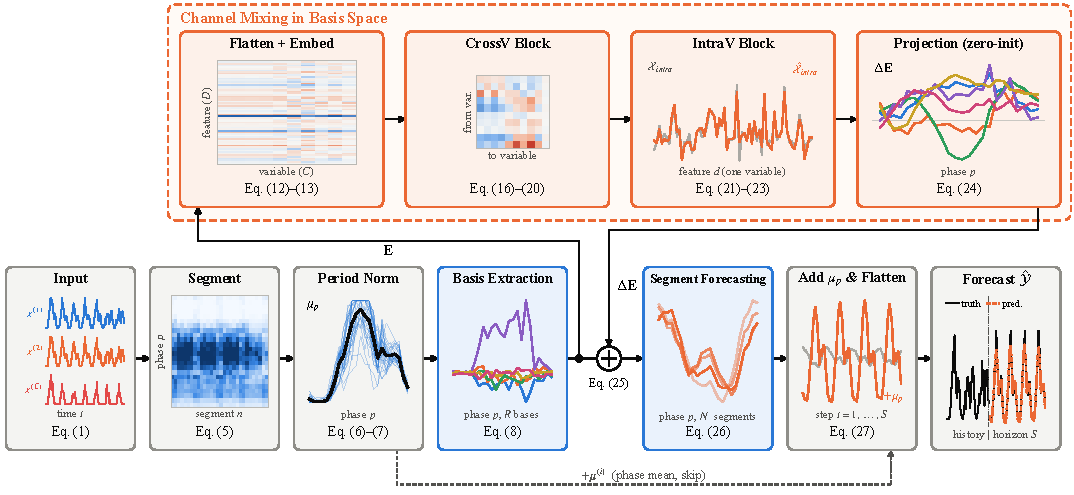
\includegraphics[width=\textwidth]{figures/dybas_architecture.pdf}
\caption{Sơ đồ tổng quan của DyBAS-Net. Mỗi biến được phân đoạn theo chu kỳ, chuẩn hóa theo pha và nén thành $R$ thành
phần cơ sở $\mathbf{E}$ (nhánh độc lập kênh). Nhánh trộn kênh học phụ thuộc liên biến trên các cơ sở đã làm phẳng và trả
về hiệu chỉnh $\Delta\mathbf{E}$ khởi tạo bằng không; các cơ sở đã hiệu chỉnh $\mathbf{E}'=\mathbf{E}+\Delta\mathbf{E}$
được ánh xạ thành các đoạn tương lai, khử chuẩn hóa và làm phẳng.}
\label{fig:model}
\end{figure*}

\subsection{Sparse Segment}
\label{sec:segment}

Theo cách nhìn dựa trên chu kỳ của SparseTSF~\cite{Lin2024SparseTSF} và TimeBase~\cite{Huang2025TimeBase}, mỗi chuỗi được
xử lý như một dãy các đoạn dài một chu kỳ thay vì từng bước thời gian riêng lẻ.

\textbf{Bước 1: Phân đoạn theo chu kỳ.} Chuỗi của biến $i$, $\mathbf{x}^{(i)}=(x^{(i)}_1,\dots,x^{(i)}_L)^{\top}$, được
sắp xếp thành \emph{ma trận đoạn} $\mathbf{X}^{(i)}\in\R^{P\times N}$ có các cột là các đoạn độ dài $P$:
\begin{equation}
\mathbf{X}^{(i)}=
\begin{bmatrix}
x^{(i)}_1 & x^{(i)}_{P+1} & \dots & x^{(i)}_{(N-1)P+1}\\
x^{(i)}_2 & x^{(i)}_{P+2} & \dots & x^{(i)}_{(N-1)P+2}\\
\vdots & \vdots & \ddots & \vdots\\
x^{(i)}_P & x^{(i)}_{2P} & \dots & x^{(i)}_{NP}
\end{bmatrix},
\label{eq:segment}
\end{equation}
tức $[\mathbf{X}^{(i)}]_{p,n}=x^{(i)}_{(n-1)P+p}$. Với ETTh1, $L=720$ và $P=24$ cho $N=30$ cột, mỗi cột là một ngày, và
$[\mathbf{X}^{(i)}]_{p,n}$ là giá trị tại giờ thứ $p$ của ngày thứ $n$: $(n-1)$ ngày trọn vẹn trước ngày $n$ chứa $(n-1)P$
điểm, đi thêm $p$ bước nữa ta đến vị trí $(n-1)P+p$ của chuỗi gốc. Khi $L$ không chia hết cho $P$, chuỗi được đệm ở đầu
bằng $NP-L$ giá trị cuối của chu kỳ đầu tiên.

\textbf{Bước 2: Chuẩn hóa theo pha.} Trung bình của mỗi hàng (pha) trên $N$ đoạn là
\begin{equation}
\mu^{(i)}_p=\frac{1}{N}\sum_{n=1}^{N}\big[\mathbf{X}^{(i)}\big]_{p,n},\qquad
\bm{\mu}^{(i)}=\big(\mu^{(i)}_1,\dots,\mu^{(i)}_P\big)^{\top}\in\R^{P},
\label{eq:phase-mean}
\end{equation}
và được trừ khỏi mọi phần tử của hàng tương ứng:
\begin{equation}
\big[\tilde{\mathbf{X}}^{(i)}\big]_{p,n}=\big[\mathbf{X}^{(i)}\big]_{p,n}-\mu^{(i)}_p .
\label{eq:period-norm}
\end{equation}
$\bm{\mu}^{(i)}$ là ``đoạn trung bình'' của biến $i$ (ví dụ phụ tải ban ngày cao hơn ban đêm); các bước sau chỉ học phần
dao động quanh nó, và $\bm{\mu}^{(i)}$ được cộng lại ở bước 8. Từ đây, mọi phép toán trên trục thời gian tác động lên $N$
đoạn thay vì $L$ điểm, và đó là nguồn gốc của tính thưa: với $L=720$ và $P=24$, trục thời gian co từ 720 điểm còn 30
đoạn.

\subsection{Pattern Extraction}
\label{sec:pattern}

\textbf{Bước 3: Trích xuất cơ sở.} Một ánh xạ tuyến tính \emph{dùng chung cho mọi biến}, với tham số học được
$\mathbf{W}_B\in\R^{N\times R}$ và $\mathbf{b}_B\in\R^{R}$, nén $N$ đoạn thành $R$ thành phần
cơ sở~\cite{Huang2025TimeBase}:
\begin{equation}
\mathbf{E}^{(i)}=\tilde{\mathbf{X}}^{(i)}\,\mathbf{W}_B+\mathbf{b}_B\in\R^{P\times R},
\label{eq:basis}
\end{equation}
trong đó $\mathbf{b}_B$ được cộng vào mọi hàng. Cột $r$ của $\mathbf{E}^{(i)}$ là một tổ hợp tuyến tính của $N$ đoạn quá
khứ $\tilde{\mathbf{x}}^{(i)}_n$ (các cột của $\tilde{\mathbf{X}}^{(i)}$), tức một ``đoạn đại diện'':
\begin{equation}
\mathbf{e}^{(i)}_r=\sum_{n=1}^{N}\big[\mathbf{W}_B\big]_{n,r}\,\tilde{\mathbf{x}}^{(i)}_n+\big[\mathbf{b}_B\big]_r
\in\R^{P}.
\label{eq:basis-col}
\end{equation}
Dựa trên tính hạng thấp của chuỗi dài~\cite{Huang2025TimeBase}, $N=30$ ngày được tóm tắt bằng $R=6$ ``ngày điển hình''.

\textbf{Ràng buộc trực giao.} Ma trận Gram tập hợp tích vô hướng giữa từng cặp thành phần cơ sở,
\begin{equation}
\mathbf{G}^{(i)}=\mathbf{E}^{(i)\top}\mathbf{E}^{(i)}\in\R^{R\times R},\qquad
\big[\mathbf{G}^{(i)}\big]_{r,s}=\big\langle\mathbf{e}^{(i)}_r,\mathbf{e}^{(i)}_s\big\rangle,
\label{eq:gram}
\end{equation}
và phần ngoài đường chéo của nó bị phạt, lấy trung bình trên $B$ mẫu của một lô và $C$ biến:
\begin{equation}
\mathcal{L}_{orth}=\frac{1}{B\,C}\sum_{b=1}^{B}\sum_{i=1}^{C}
\big\|\mathbf{G}^{(i)}_b-\operatorname{diag}\big(\mathbf{G}^{(i)}_b\big)\big\|_F .
\label{eq:orth}
\end{equation}
$\mathcal{L}_{orth}=0$ khi các thành phần cơ sở đôi một trực giao, nên mỗi thành phần mang một kiểu biến thiên riêng,
không dư thừa. Số hạng này chỉ dùng khi huấn luyện; khi đánh giá chỉ dùng MSE và MAE. Ma trận cơ sở $\mathbf{E}^{(i)}$
chỉ gồm $P\cdot R$ số (ví dụ $24\times6=144$ thay vì 720), và DyBAS-Net học phụ thuộc liên biến chính trên các mẫu hình
đã trích xuất này.

\subsection{Dynamic Dependency}
\label{sec:dependency}

Bước 4--7 tạo thành nhánh trộn kênh. CrossVBlock, DropFusion và IntraVBlock được lấy từ
DyTimeNet~\cite{Chen2026DyTimeNet}; phép mã hóa ở bước 4 và phép chiếu ngược ở bước 7 là phần mới, cho phép nhánh này
hoạt động trên các hệ số cơ sở thay vì các điểm thời gian gốc.

\textbf{Bước 4: Mã hóa cơ sở.} Mỗi $\mathbf{E}^{(i)}$ được làm phẳng theo hàng thành một vector, và $C$ biến được xếp
thành ma trận $\bar{\mathbf{E}}\in\R^{PR\times C}$:
\begin{equation}
\mathbf{e}^{(i)}=\vecr\big(\mathbf{E}^{(i)}\big)\in\R^{PR},\quad
\bar{\mathbf{E}}=\big[\mathbf{e}^{(1)},\dots,\mathbf{e}^{(C)}\big].
\label{eq:flatten}
\end{equation}
Một phép chiếu tuyến tính với tham số học được $\mathbf{W}_{enc}\in\R^{PR\times D}$ và bias $\mathbf{b}_{enc}\in\R^{D}$
(cộng vào mọi cột) ánh xạ chúng sang không gian ẩn $D$ chiều:
\begin{equation}
\mathcal{X}_{enc}=\mathbf{W}_{enc}^{\top}\,\bar{\mathbf{E}}+\mathbf{b}_{enc}\in\R^{D\times C}.
\label{eq:embed}
\end{equation}
Khác với lớp embedding của DyTimeNet vốn chiếu $L$ điểm gốc của mỗi biến~\cite{Chen2026DyTimeNet}, đầu vào ở đây gồm
$PR$ hệ số cơ sở.

\textbf{LayerNorm và GELU.} LayerNorm~\cite{Ba2016LayerNorm} chuẩn hóa $D$ đặc trưng của mỗi biến (một cột
$\mathbf{h}\in\R^{D}$), đưa mọi biến về cùng thang đo trước khi trộn:
\begin{equation}
\LN(\mathbf{h})=\bm{\gamma}\odot\frac{\mathbf{h}-\mu_{\mathbf{h}}}{\sqrt{\sigma^2_{\mathbf{h}}+\varepsilon}}+\bm{\beta},
\label{eq:ln-def}
\end{equation}
trong đó $\mu_{\mathbf{h}}$ và $\sigma^2_{\mathbf{h}}$ là trung bình và phương sai các phần tử của $\mathbf{h}$, còn
$\bm{\gamma},\bm{\beta}\in\R^{D}$ là tham số học được. Hàm kích hoạt là GELU~\cite{Hendrycks2016GELU},
\begin{equation}
\GELU(x)=x\cdot\Phi(x)=\frac{x}{2}\Big(1+\operatorname{erf}\Big(\frac{x}{\sqrt{2}}\Big)\Big),
\label{eq:gelu}
\end{equation}
với $\Phi$ là hàm phân phối tích lũy của $\mathcal{N}(0,1)$ và
$\operatorname{erf}(x)=\frac{2}{\sqrt{\pi}}\int_0^x e^{-t^2}dt$.

\textbf{Bước 5: Khối liên biến (CrossVBlock).} Sau chuẩn hóa,
$\tilde{\mathcal{X}}_{enc}=\LN(\mathcal{X}_{enc})\in\R^{D\times C}$, một MLP nút thắt dọc trục biến $C\to C'\to C$ với
$\mathbf{W}_{df,1}\in\R^{C\times C'}$ và $\mathbf{W}_{df,2}\in\R^{C'\times C}$ (bias $\mathbf{b}_1$, $\mathbf{b}_2$ cộng
vào mọi hàng) tính, khi kiểm tra,
\begin{align}
\mathbf{H}&=\GELU\big(\tilde{\mathcal{X}}_{enc}\,\mathbf{W}_{df,1}+\mathbf{b}_1\big)\in\R^{D\times C'},\label{eq:cross1}\\
\mathcal{X}_{cross}&=\mathbf{H}\,\mathbf{W}_{df,2}+\mathbf{b}_2\in\R^{D\times C}.\label{eq:cross2}
\end{align}
Mỗi \emph{hàng} của $\tilde{\mathcal{X}}_{enc}$ chứa một đặc trưng của cả $C$ biến, nên phép nhân phải với $\mathbf{W}_{df}$ tạo
mỗi biến mới là tổ hợp của mọi biến trên đặc trưng đó, tức trộn thông tin \emph{giữa} các biến. Khi huấn luyện, hai lớp
tuyến tính này được thay bằng các lớp DropFusion~\cite{Chen2026DyTimeNet}.

\textbf{DropFusion: mặt nạ cạnh $\mathcal{M}_1$ và mặt nạ nút $\mathcal{M}_2$.} Xét lớp thứ nhất (đầu vào
$\tilde{\mathcal{X}}_{enc}\in\R^{D\times C}$, trọng số $\mathbf{W}_{df,1}\in\R^{C\times C'}$). Ở giai đoạn thứ nhất, một
\emph{mặt nạ cạnh} $\mathcal{M}_1\in\{0,1\}^{C\times C'}$, với mỗi phần tử bằng 0 với xác suất $p_1$, xóa kết nối giữa
một biến đầu vào và một nút ẩn; mặt nạ được lấy mẫu lại cho mỗi lô:
\begin{equation}
\mathbf{W}_{masked}=\mathbf{W}_{df,1}\odot\mathcal{M}_1 .
\label{eq:wmasked}
\end{equation}
Ở giai đoạn thứ hai, một \emph{mặt nạ nút} $\mathcal{M}_2\in\{0,1\}^{D\times C'}$, với mỗi phần tử bằng 0 với xác suất
$p_2$, tắt ngẫu nhiên từng đầu ra; mặt nạ được lấy mẫu riêng cho từng mẫu:
\begin{equation}
\mathbf{Y}_{masked}=\big(\tilde{\mathcal{X}}_{enc}\,\mathbf{W}_{masked}+\mathbf{b}_1\big)\odot\mathcal{M}_2 .
\label{eq:ymasked}
\end{equation}
Lớp thứ hai được xử lý tương tự, với đầu vào $\mathbf{H}$ và trọng số $\mathbf{W}_{df,2}$.

\textbf{DropFusion: chuẩn hóa kỳ vọng.} Khi huấn luyện, một phần kết nối bị tắt theo $p_1$ và $p_2$, còn khi kiểm tra mọi
kết nối đều hoạt động, nên tổng tín hiệu sẽ tăng lên và làm lệch đầu ra. Các hệ số bù giữ kỳ vọng tín hiệu như nhau ở cả
hai giai đoạn, cho ta lớp DropFusion hoàn chỉnh dùng khi huấn luyện:
\begin{equation}
\DF(\tilde{\mathcal{X}}_{enc})=\frac{1}{1-p_2}\Big[\frac{\tilde{\mathcal{X}}_{enc}\,(\mathbf{W}_{df,1}\odot\mathcal{M}_1)}{1-p_1}
+\mathbf{b}_1\Big]\odot\mathcal{M}_2 .
\label{eq:dropfusion}
\end{equation}
Khi kiểm tra, $\mathcal{M}_1=\mathcal{M}_2=\one$, không áp dụng hệ số bù, và lớp này trở về lớp tuyến tính
của \eqref{eq:cross1}--\eqref{eq:cross2}.

Phụ thuộc học được là \emph{thưa} vì mỗi bước huấn luyện chỉ thấy một tập con ngẫu nhiên các cạnh giữa các biến, ngăn mô
hình dựa vào bất kỳ tương quan đơn lẻ nào, vốn có thể là tương quan giả. Phụ thuộc là \emph{động} vì đồ thị phụ thuộc thưa
thay đổi ở mỗi bước và các đặc trưng được trộn được tính từ các thành phần cơ sở của cửa sổ hiện tại, nên ảnh hưởng của
một biến lên biến khác thay đổi theo từng mẫu.

\textbf{Bước 6: Khối nội biến (IntraVBlock).} Một kết nối tắt cộng đặc trưng liên biến vào đặc trưng đã chuẩn hóa để giữ
thông tin gốc của mỗi biến:
\begin{equation}
\mathcal{X}_{intra}=\mathcal{X}_{cross}+\tilde{\mathcal{X}}_{enc}\in\R^{D\times C}.
\label{eq:cross-res}
\end{equation}
Một mạng truyền thẳng dùng chung cho mọi biến được áp dụng lên \emph{từng cột} (biến) $\mathbf{h}\in\R^{D}$,
\begin{equation}
\FFN(\mathbf{h})=\mathbf{W}_4\,\GELU(\mathbf{W}_3\mathbf{h}+\mathbf{b}_3)+\mathbf{b}_4,
\label{eq:ffn}
\end{equation}
với $\mathbf{W}_3\in\R^{D_{ff}\times D}$ và $\mathbf{W}_4\in\R^{D\times D_{ff}}$, có LayerNorm phía trước và kết nối tắt
phía sau:
\begin{equation}
\hat{\mathcal{X}}_{intra}=\mathcal{X}_{intra}+\FFN\big(\LN(\mathcal{X}_{intra})\big)\in\R^{D\times C}.
\label{eq:intra}
\end{equation}
Dropout được áp dụng bên trong FFN khi huấn luyện.

\textbf{Bước 7: Chiếu ngược và hiệu chỉnh cơ sở.} Biểu diễn ẩn được chiếu ngược về không gian cơ sở,
\begin{equation}
\Delta\bar{\mathbf{E}}=\mathbf{W}_{out}^{\top}\,\hat{\mathcal{X}}_{intra}+\mathbf{b}_{out}\in\R^{PR\times C},
\qquad \mathbf{W}_{out}\in\R^{D\times PR},
\label{eq:proj}
\end{equation}
cột $i$ được định hình lại thành $\Delta\mathbf{E}^{(i)}\in\R^{P\times R}$, và hiệu chỉnh được cộng vào các cơ sở:
\begin{equation}
\mathbf{E}'^{(i)}=\mathbf{E}^{(i)}+\Delta\mathbf{E}^{(i)}.
\label{eq:correct}
\end{equation}
$\mathbf{W}_{out}$ và $\mathbf{b}_{out}$ được khởi tạo bằng không, nên $\Delta\mathbf{E}^{(i)}=\mathbf{0}$ khi bắt đầu
huấn luyện và DyBAS-Net trùng với backbone độc lập kênh của nó. Vì vậy nhánh trộn chỉ học một \emph{hiệu chỉnh}: nó dùng
thông tin của các biến khác để điều chỉnh các ``ngày điển hình'' của biến $i$, và không thể khiến mô hình xuất phát từ một
điểm kém hơn backbone.


\textbf{Bước 8: Dự báo đoạn và tái tạo chuỗi.} Một ánh xạ tuyến tính dùng chung sinh $N'$ đoạn tương lai từ $R$ cơ sở đã
hiệu chỉnh,
\begin{equation}
\hat{\mathbf{Y}}^{(i)}=\mathbf{E}'^{(i)}\,\mathbf{W}_F+\mathbf{b}_F\in\R^{P\times N'},\qquad
\mathbf{W}_F\in\R^{R\times N'}.
\label{eq:forecast}
\end{equation}
Trung bình pha được cộng lại vào mọi đoạn tương lai, và các cột được nối thành một chuỗi, giữ lại $S$ bước đầu:
\begin{equation}
\hat{x}^{(i)}_{L+t}=\big[\hat{\mathbf{Y}}^{(i)}\big]_{p,n}+\mu^{(i)}_p,\qquad t=(n-1)P+p,\;\; t=\overline{1,S}.
\label{eq:merge}
\end{equation}
Ghép tất cả các biến cho $\hat{\mathcal{Y}}\in\R^{S\times C}$. Bỏ bước 4--7 ($\mathbf{E}'^{(i)}=\mathbf{E}^{(i)}$) ta thu
lại TimeBase~\cite{Huang2025TimeBase}.

\textbf{Điều chỉnh trọng số và tối ưu.} Các trọng số được cập nhật ngược hướng gradient của hàm mục
tiêu~\eqref{eq:objective}; ở dạng cơ bản,
\begin{equation}
\bm{\theta}_{k+1}=\bm{\theta}_k-\alpha\,\frac{\partial\mathcal{L}}{\partial\bm{\theta}_k},
\label{eq:gd}
\end{equation}
với $\bm{\theta}$ gồm mọi trọng số $\mathbf{W}$ và bias $\mathbf{b}$ và $k$ là bước cập nhật; trong thực tế dùng bộ tối ưu Adam~\cite{Kingma2014Adam}. Hai tốc độ học được sử dụng: $\alpha=\alpha_B$ cho backbone
$\mathbf{W}_B,\mathbf{b}_B,\mathbf{W}_F,\mathbf{b}_F$, và $\alpha=\alpha_M$ cho nhánh trộn. Tại epoch $\tau$, tốc độ học giữ
nguyên trong bốn epoch đầu, sau đó nhân với $0{,}8$ mỗi epoch,
\begin{equation}
\alpha^{(\tau)}=\begin{cases}\alpha, & \tau\le4,\\ \alpha\cdot0.8^{\,\tau-4}, & \tau>4.\end{cases}
\label{eq:lr}
\end{equation}
Huấn luyện dừng sớm khi MSE trên tập kiểm định không cải thiện trong năm epoch, và giữ lại bộ trọng số có MSE kiểm định
thấp nhất.

\textbf{Độ phức tạp.} Với mỗi mẫu, backbone (\eqref{eq:basis} và \eqref{eq:forecast}) cần $CPR(N+N')$ phép
nhân--cộng (MACs), còn nhánh trộn cần
\begin{equation}
\text{MACs}_M=\underbrace{2CPRD}_{\text{mã hóa/chiếu}}+\underbrace{2DCC'}_{\text{CrossV}}
+\underbrace{2CDD_{ff}}_{\text{IntraV}} .
\label{eq:macs}
\end{equation}
Không có số hạng nào tỉ lệ với $L\cdot S$; nhánh trộn không phụ thuộc vào $L$ hay $S$. Với Electricity ($C=321$,
$L=S=720$, $P=24$, $R=6$, $D=64$), backbone cần khoảng 2,8M MACs và nhánh trộn khoảng 21,0M, tổng cộng 23,8M, trong khi
DLinear cần $2CLS\approx333$M MACs.

\subsection{Proposed Model: DyBAS-Net}
\label{sec:model}



\section{Experiments}
\label{sec:exp}



\section{Conclusion}
\label{sec:conclusion}


\bibliographystyle{IEEEtran}
\bibliography{references}

\end{document}
